\chapter{MARCO METODOLÓGICO (DEL PROCESO DE DISEÑO)}
\label{cap:metodologia}

\section{Selección y descripción de la metodología de diseño y estrategia de validación}
\label{sec:metodo-diseno}

El desarrollo se organizó según el modelo de desarrollo de productos de VDI 2221, parte 1 \cite{vdi2221}. Este enfoque permitió separar la necesidad del taller de la configuración elegida para atenderla. Primero se identificaron las funciones y restricciones; después se compararon conceptos y se desarrollaron sus componentes. La revisión de los cálculos y de las interferencias permitió volver sobre decisiones anteriores cuando aparecieron incompatibilidades.

La aplicación del método se concentró en dos subsistemas relacionados: el soporte y posicionamiento del rodamiento, y la aplicación y recogida del fluido. La geometría de la pieza condicionó los apoyos y el acceso de las boquillas. A su vez, la trayectoria del aplicador exigió reservar espacio en el bastidor y en la cabina. Por ello, las decisiones sobre estructura y limpieza se revisaron de manera coordinada, aunque su dimensionamiento se efectuó con modelos distintos.

La Tabla~\ref{tab:oe_metodo_revision} relaciona las actividades con los cinco objetivos específicos formulados en la introducción, junto con la herramienta empleada y la forma de comprobar su resultado, y la Figura~\ref{fig:metodo_revision} resume la secuencia del proceso y su retorno a las decisiones que requieren ajuste. Las decisiones se explican en este capítulo, los cálculos se desarrollan en el Capítulo~\ref{cap:diseno} y los resultados se contrastan en el Capítulo~\ref{cap:resultados}.

\begingroup
\small\singlespacing
\setlength{\parskip}{0pt}
\setlength{\tabcolsep}{4pt}
\renewcommand{\arraystretch}{1.1}
\begin{longtable}{@{}>{\raggedright\arraybackslash}p{0.9cm}>{\raggedright\arraybackslash}p{\dimexpr(\textwidth-0.9cm-6\tabcolsep)*35/100\relax}>{\raggedright\arraybackslash}p{\dimexpr(\textwidth-0.9cm-6\tabcolsep)*35/100\relax}>{\raggedright\arraybackslash}p{\dimexpr(\textwidth-0.9cm-6\tabcolsep)*30/100\relax}@{}}
\caption{Relación entre objetivos específicos, actividades, herramientas y comprobación}\label{tab:oe_metodo_revision}\\
\toprule
\textbf{Obj.} & \textbf{Actividad realizada} & \textbf{Herramienta y salida} & \textbf{Comprobación}\\
\midrule\endfirsthead
\caption[]{Relación entre objetivos específicos, actividades, herramientas y comprobación (continuación)}\\
\toprule
\textbf{Obj.} & \textbf{Actividad realizada} & \textbf{Herramienta y salida} & \textbf{Comprobación}\\
\midrule\endhead
\midrule\multicolumn{4}{r}{\textit{Continúa en la página siguiente.}}\\\endfoot
\bottomrule\endlastfoot
OE1 & Se organizaron los datos del rodamiento, las necesidades de mantenimiento y las restricciones del taller. & Ficha del fabricante y análisis del entorno; especificaciones E01--E14. & Trazabilidad de cada especificación a su origen (Tabla~\ref{tab:especificaciones_revision}).\\
OE2 & Se descompuso la operación en funciones y se combinaron principios de soporte, movimiento y aplicación del fluido. & Matriz morfológica; cuatro alternativas integradas. & Filtros pasa/no pasa (Tabla~\ref{tab:filtros_revision}).\\
OE3 & Se aplicó una matriz ponderada de ocho criterios y se analizó el compromiso con la segunda alternativa. & Matriz de decisión; arquitectura seleccionada. & Diferencia de puntaje y sensibilidad al peso del costo.\\
OE4 & Se dimensionaron el soporte, el traslado, el distribuidor y la red hidráulica, y se seleccionaron componentes. & Cálculo analítico, SAP2000, CalculiX, SolidWorks, guiones en Python, CAD paramétrico y planos. & Contraste manual--modelo y reproducción del caso de cálculo.\\
OE5 & Se evaluó el desempeño calculado y simulado, y se reajustaron geometría y componentes. & CFD (ANSYS Fluent y OpenFOAM), trazado de rayos, barridos CAD y presupuesto de tolerancias. & Verificación numérica, caso puente entre programas y detección de interferencias.\\
\end{longtable}
\endgroup

\begin{figure}[htbp]
\centering
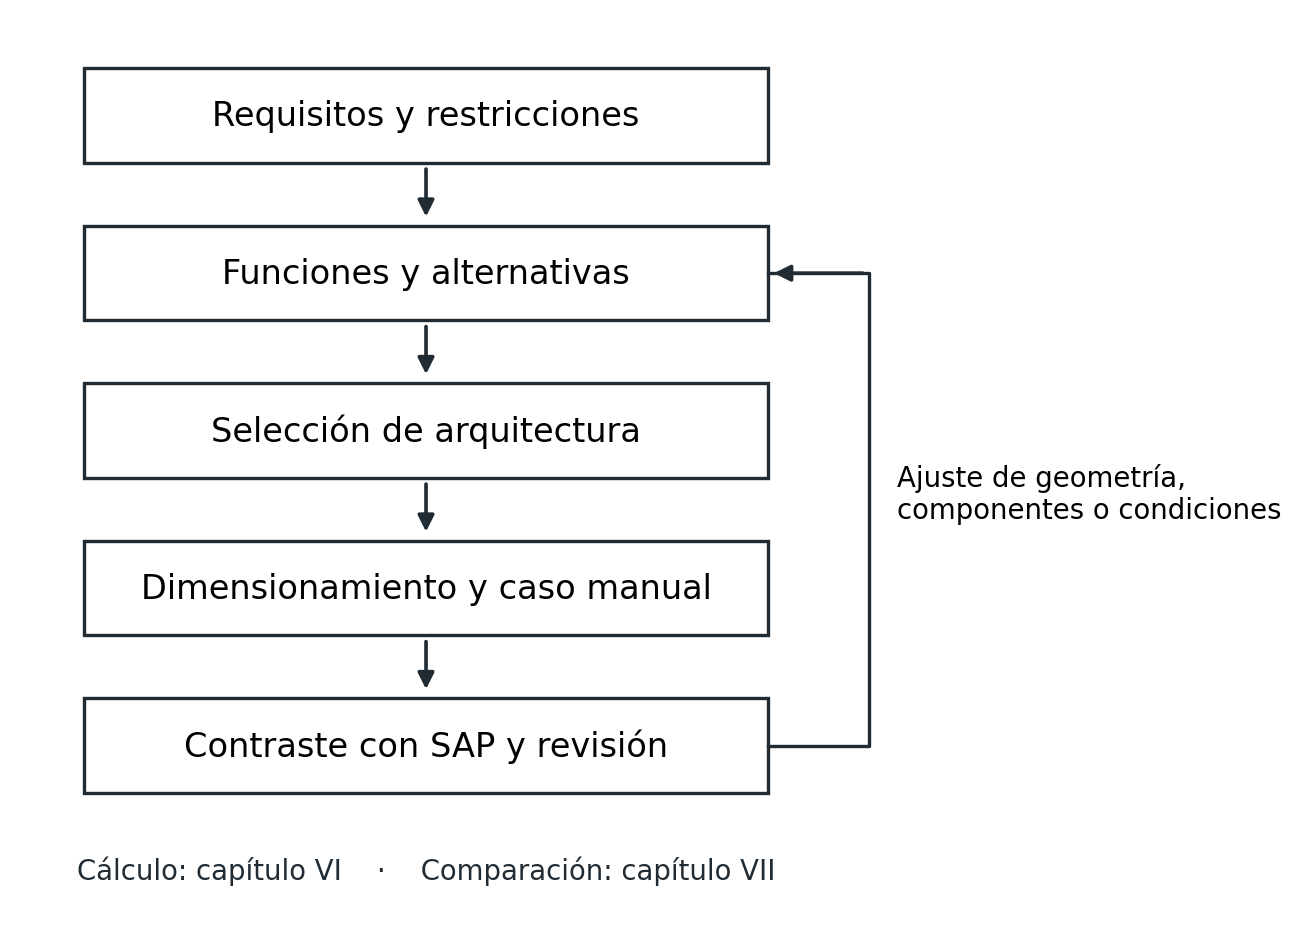
\includegraphics[width=0.93\textwidth]{images/proceso_metodologico}
\caption{Organización del proceso de diseño y retorno a las decisiones que requieren ajuste. Elaboración propia.}
\label{fig:metodo_revision}
\end{figure}

En el soporte se escogió un caso centrado con tres apoyos del rodamiento, cuyas reacciones verticales pueden obtenerse con las tres ecuaciones de equilibrio; ese desarrollo manual sirvió de control del modelo estructural. En la aspersión se definió una cadena que relaciona superficies objetivo, boquillas, caudal simultáneo, pérdidas del circuito y punto de bombeo, y que luego se contrastó con la simulación del mojado.

Las herramientas de modelado se eligieron según la pregunta que debía responder cada una. La Tabla~\ref{tab:herramientas} justifica cada herramienta e indica la verificación que se le aplicó.

\begingroup
\small\singlespacing
\setlength{\parskip}{0pt}
\setlength{\tabcolsep}{4pt}
\renewcommand{\arraystretch}{1.1}
\begin{longtable}{@{}>{\raggedright\arraybackslash}p{2.7cm}>{\raggedright\arraybackslash}p{\dimexpr(\textwidth-2.7cm-6\tabcolsep)/3\relax}>{\raggedright\arraybackslash}p{\dimexpr(\textwidth-2.7cm-6\tabcolsep)/3\relax}>{\raggedright\arraybackslash}p{\dimexpr(\textwidth-2.7cm-6\tabcolsep)/3\relax}@{}}
\caption{Herramientas de modelado, necesidad que atienden y verificación aplicada}\label{tab:herramientas}\\
\toprule
\textbf{Herramienta} & \textbf{Necesidad} & \textbf{Justificación} & \textbf{Verificación}\\
\midrule\endfirsthead
\caption[]{Herramientas de modelado, necesidad que atienden y verificación aplicada (continuación)}\\
\toprule
\textbf{Herramienta} & \textbf{Necesidad} & \textbf{Justificación} & \textbf{Verificación}\\
\midrule\endhead
\midrule\multicolumn{4}{r}{\textit{Continúa en la página siguiente.}}\\\endfoot
\bottomrule\endlastfoot
SAP2000 24.2.0 y 27.1 & Respuesta global del bastidor de perfiles y del soporte superior del distribuidor. & Modelo de barras con comprobación AISC 360-16 \cite{csi_analisis_2016,aisc360}. & Equilibrio contrastado con el cálculo manual; tablas exportadas.\\
FreeCAD FEM, Gmsh y CalculiX & Flexión local de los soportes de los centradores, que un modelo de barras no capta. & Elementos sólidos sobre la geometría real del perfil y las placas \cite{shigley2015}. & Dos niveles de malla, ambos signos de carga y control de equilibrio.\\
CalculiX y parrilla de pared delgada en Python & Torsión del bastidor de perfiles abiertos; el modelo de barras solo representa la torsión uniforme. & Torsión no uniforme con alabeo \cite{aiscdg9}. & Casos de control analíticos y cálculo independiente.\\
Guiones en Python & Red hidráulica iterativa, trazado de rayos y posproceso del CFD. & Cálculo reproducible y trazable. & Reproducción exacta del caso de cálculo manual.\\
ANSYS Fluent 2026 R1 & Mojado y dosis de la configuración base de 22 boquillas y de la configuración inferior de 24 boquillas. & Fase discreta lagrangiana acoplada al aire \cite{fluent2026}. & Tres mallas, paso de tiempo, dominio, número de parcelas y caso puente.\\
OpenFOAM v2606 & Mojado del agujero con las boquillas de la lanza; impacto local de una lámina con volumen de fluido (interFoam). & Mismo modelo físico en código abierto; volumen de fluido para la película \cite{deshpande2012}. & Caso puente con Fluent; cuatro mallas en el impacto local.\\
FreeCAD 1.1 (CAD) & Geometría, masas, interferencias y barridos del conjunto. & Modelo paramétrico regenerable por guiones. & Barridos de traslado, giro, retirada de la lanza y accionamiento; auditoría de solapes.\\
SolidWorks 2024 & Planos normalizados, detección de interferencias y verificaciones locales de piezas. & Herramienta de dibujo con símbolos ISO de soldadura y estudios estáticos de sólidos. & Cotas contrastadas con el CAD; segunda revisión de interferencias.\\
\end{longtable}
\endgroup

El CFD se ejecutó en ANSYS Fluent. Antes de ampliar el dominio se repitió en Fluent el caso del agujero ya resuelto en OpenFOAM; ese caso puente permitió comprobar que el cambio de programa no alteraba el resultado en esa superficie (Sección~\ref{sec:resultados-aspersion}). Las simulaciones de Fluent las ejecutó el segundo autor.

\paragraph{Uso de herramientas de inteligencia artificial.} Se usaron asistentes basados en inteligencia artificial en cuatro tareas. La primera fue programar guiones de cálculo y de posproceso, y guiones que generaron por interfaz de programación los modelos de SAP2000, el modelo CAD en FreeCAD y los planos en SolidWorks. La segunda fue revisar de forma independiente cálculos y la coherencia de los datos entre archivos. La tercera fue proponer alternativas de diseño, que los autores decidieron o confirmaron. La cuarta fue preparar borradores de texto y de tablas de este informe a partir de los archivos del proyecto. Los autores definieron el problema y los criterios, tomaron las decisiones de diseño y son responsables del contenido. Los guiones y sus salidas se conservan en el Anexo~\ref{anx:programas}, de modo que cada resultado puede reproducirse sin el asistente.

La estrategia de validación se basó en la verificación numérica de cada modelo (equilibrio, convergencia de malla, paso de tiempo y dominio) y en el contraste cruzado entre métodos independientes, cuyos escenarios se desarrollan en la Sección~\ref{sec:plan-pruebas}. Cada resultado se verificó por simulación o por cálculo; ninguno se validó con ensayos. La comprobación experimental de la huella de la boquilla, de la remoción del contaminante, del traslado y del bloqueo queda fuera del alcance de la tesis.

\section{Formulación de especificaciones técnicas}

Las necesidades se tradujeron en dimensiones, cargas, condiciones funcionales y criterios de aceptación. Se distinguieron los datos impuestos por el rodamiento, los criterios adoptados por el proyecto y las metas propuestas para el subsistema de limpieza. Las dimensiones de un perfil o la ubicación final de un mecanismo no se trataron como necesidades del usuario, pues corresponden a decisiones que se justifican durante el dimensionamiento.

Las metas del subsistema de aspersión E09--E13 proceden de la especificación de requerimientos que el equipo elaboró a partir de la reunión técnica con la empresa de remanufactura de referencia. Esa especificación se redactó para una arquitectura anterior del aplicador, por lo que se conservaron solo los requisitos funcionales y de desempeño que no dependen de ella. La Tabla~\ref{tab:especificaciones_revision} asigna a cada especificación su origen, su estado y su método de comprobación.

\begingroup
\small\singlespacing
\setlength{\parskip}{0pt}
\setlength{\tabcolsep}{4pt}
\renewcommand{\arraystretch}{1.1}
\begin{longtable}{@{}>{\raggedright\arraybackslash}p{1.0cm}>{\raggedright\arraybackslash}p{\dimexpr(\textwidth-1.0cm-6\tabcolsep)*40/100\relax}>{\raggedright\arraybackslash}p{\dimexpr(\textwidth-1.0cm-6\tabcolsep)*25/100\relax}>{\raggedright\arraybackslash}p{\dimexpr(\textwidth-1.0cm-6\tabcolsep)*35/100\relax}@{}}
\caption{Especificaciones técnicas, origen y método de comprobación}\label{tab:especificaciones_revision}\\
\toprule
\textbf{Cód.} & \textbf{Requisito o meta} & \textbf{Origen y estado} & \textbf{Método de comprobación}\\
\midrule\endfirsthead
\caption[]{Especificaciones técnicas, origen y método de comprobación (continuación)}\\
\toprule
\textbf{Cód.} & \textbf{Requisito o meta} & \textbf{Origen y estado} & \textbf{Método de comprobación}\\
\midrule\endhead
\midrule\multicolumn{4}{r}{\textit{Continúa en la página siguiente.}}\\\endfoot
\bottomrule\endlastfoot
\multicolumn{4}{@{}l}{\textit{Soporte y posicionamiento}}\\
E01 & Admitir el rodamiento de diámetro exterior 1420 mm, agujero de 900 mm y ancho de 515 mm. & Ficha del fabricante \cite{skf241}. & Envolvente de la pieza en el modelo.\\
E02 & Recibir una masa de rodamiento de 3032 kg y considerar por separado los pesos de estructura y accesorios. & Ficha del fabricante. & Balance de masas y correspondencia con las cargas de cada cálculo.\\
E03 & Mantener la flecha relativa del miembro evaluado dentro de $L/800$. & Criterio propuesto; L/360 y L/1000 se informan como referencia. & Desplazamiento respecto de la cuerda de sus extremos.\\
E04 & Relación demanda/capacidad no mayor que uno bajo las combinaciones declaradas. & AISC 360-16 \cite{aisc360}. & Resumen de diseño de acero; uniones por separado.\\
E05 & Transmitir reacciones normales compresivas en las interfaces sin amarre vertical. & Condición física del contacto. & Equilibrio y factibilidad del contacto.\\
E06 & Error radial de colocación del rodamiento no mayor que 5 mm. & Criterio del proyecto. & Presupuesto de tolerancias sobre el modelo, por nivel de fuerza del centrador.\\
E07 & Permitir la carga exterior y mantener la mesa inmovilizada durante el lavado. & Requisito funcional. & Envolventes de movimiento, bloqueo y secuencia.\\
E08 & Carrera de captura del centrador no menor que 5 mm después de tolerancias, con excentricidad inicial de 5 mm en cualquier dirección. & Criterio del proyecto. & Barridos de captura y presupuesto de tolerancias.\\
\multicolumn{4}{@{}l}{\textit{Aplicación del fluido}}\\
E09 & Presión en la toma de cada boquilla entre 4 y 6 bar (admisible entre 2 y 8 bar). & Especificación del subsistema de aspersión. & Red hidráulica.\\
E10 & Presión de aplicación no mayor que 8 bar, para preservar las pistas. & Especificación del subsistema de aspersión. & Red hidráulica.\\
E11 & Velocidad en la tubería de impulsión entre 1 y 3 m/s. & Especificación del subsistema de aspersión. & Red hidráulica.\\
E12 & Velocidad del rotor entre 1 y 2 rpm (admisible entre 0,5 y 5 rpm) y tiempo por vuelta entre 30 y 60 s. & Especificación del subsistema de aspersión. & Valor de operación del aplicador.\\
E13 & Cobertura geométrica de las superficies exteriores y del agujero de al menos 80\,\% (mínimo) y 95\,\% (objetivo). & Especificación del subsistema de aspersión. & Trazado de rayos y CFD.\\
\multicolumn{4}{@{}l}{\textit{Integración}}\\
E14 & Holgura positiva entre la mesa y el aplicador en traslado y giro. & Requisito funcional. & Barridos CAD.\\
\end{longtable}
\endgroup

Todas las especificaciones se comprueban por cálculo, simulación o modelo CAD, que es el alcance de la tesis. El modelo de mojado mide el líquido que llega a cada superficie y no el desprendimiento de la grasa, por lo que la especificación del subsistema no incluye metas de remoción.

\section{Descripción técnica de múltiples restricciones realistas}
\label{sec:filtros-diseno}

Las restricciones RS-01--RS-12 del Capítulo~\ref{cap:marco-referencial} se convirtieron en reglas de admisión para las alternativas. Un concepto que incumpla una condición indispensable no puede compensar ese incumplimiento con una nota alta en costo o simplicidad. Cuando falta el dato necesario para aplicar un filtro, la decisión se conserva abierta hasta disponer de la evidencia correspondiente. No se estableció como exclusión general el giro del rodamiento: las arquitecturas con giro se conservaron para compararlas, siempre que incorporaran soporte, sujeción y protección compatibles con la masa.

La Tabla~\ref{tab:filtros_revision} muestra la regla de admisión de cada restricción y su resultado para las cuatro alternativas.

\begingroup
\small\singlespacing
\setlength{\parskip}{0pt}
\setlength{\tabcolsep}{4pt}
\renewcommand{\arraystretch}{1.1}
\begin{longtable}{@{}>{\raggedright\arraybackslash}p{2.3cm}>{\raggedright\arraybackslash}p{\dimexpr(\textwidth-2.3cm-4\tabcolsep)*55/100\relax}>{\raggedright\arraybackslash}p{\dimexpr(\textwidth-2.3cm-4\tabcolsep)*45/100\relax}@{}}
\caption{Aplicación de restricciones como filtros de diseño}\label{tab:filtros_revision}\\
\toprule
\textbf{Restricción} & \textbf{Regla de admisión} & \textbf{Resultado para A1--A4}\\
\midrule\endfirsthead
\caption[]{Aplicación de restricciones como filtros de diseño (continuación)}\\
\toprule
\textbf{Restricción} & \textbf{Regla de admisión} & \textbf{Resultado para A1--A4}\\
\midrule\endhead
\midrule\multicolumn{3}{r}{\textit{Continúa en la página siguiente.}}\\\endfoot
\bottomrule\endlastfoot
RS-02 Masa y geometría & Se excluye la configuración que no admite la carga o la envolvente requeridas. & Pasan las cuatro; A1 y A4 condicionadas a una sujeción para giro compatible con 3032 kg.\\
RS-03 Preservación y acceso & Se modifica o excluye el concepto que obstruye una zona requerida o transmite carga por una superficie no prevista. & Pasan las cuatro a nivel funcional; la cobertura se verifica en el Capítulo~\ref{cap:resultados}.\\
RS-04--RS-05 Izaje, espacio y losa & Se excluye una disposición con interferencia; sin levantamiento de planta, la aptitud final depende de ese dato. & Condicionadas para las cuatro (requieren datos de planta).\\
RS-01, RS-11 Movimiento y bloqueo & Se excluye una secuencia que requiere lavar con la mesa sin inmovilizar o intervenir en una zona de movimiento peligroso. & Pasan las cuatro con inmovilización durante el lavado.\\
RS-08--RS-09 Contención y fluido & Se excluye una propuesta cuya operación depende de descargar el fluido sin una gestión definida. & Pasan las cuatro con cabina, bandeja y recolección.\\
RS-10 Recursos económicos & Un presupuesto máximo se aplica como filtro solo si está documentado. & No aplicado como filtro (sin techo acreditado); el costo es criterio comparativo.\\
\end{longtable}
\endgroup

La aplicación de estos filtros distinguió una incompatibilidad demostrada de una selección que exige completar datos. Una capacidad publicada inferior a la masa de la pieza permitió descartar esa versión de equipo en el Capítulo~\ref{cap:estado-arte}; en cambio, la ausencia de una cotización no demuestra que una arquitectura sea inviable, solo impide cerrar su evaluación económica.

\section{Generación y selección de alternativas mediante matriz de decisión}

\subsection{Generación de alternativas}

El análisis funcional partió de cinco acciones: recibir el rodamiento, sostenerlo y posicionarlo, exponer sus superficies al medio de limpieza, aplicar el fluido y recoger el residuo. Se distinguió el movimiento necesario para cargar la máquina del movimiento utilizado durante el lavado. Esta separación evitó interpretar una pieza inmóvil durante la limpieza como una mesa que no puede salir de la cabina.

La Tabla~\ref{tab:morfologica_revision} organiza los principios de solución considerados. Las opciones de cada fila representan formas de realizar una función; su combinación se revisó para obtener máquinas completas y evitar conjuntos incompatibles.

\begingroup
\small\singlespacing
\setlength{\parskip}{0pt}
\setlength{\tabcolsep}{4pt}
\renewcommand{\arraystretch}{1.1}
\begin{longtable}{@{}>{\raggedright\arraybackslash}p{2.6cm}>{\raggedright\arraybackslash}p{\dimexpr(\textwidth-2.6cm-6\tabcolsep)/3\relax}>{\raggedright\arraybackslash}p{\dimexpr(\textwidth-2.6cm-6\tabcolsep)/3\relax}>{\raggedright\arraybackslash}p{\dimexpr(\textwidth-2.6cm-6\tabcolsep)/3\relax}@{}}
\caption{Principios de solución utilizados para generar alternativas}\label{tab:morfologica_revision}\\
\toprule
\textbf{Función} & \textbf{Opción 1} & \textbf{Opción 2} & \textbf{Opción 3}\\
\midrule\endfirsthead
\caption[]{Principios de solución utilizados para generar alternativas (continuación)}\\
\toprule
\textbf{Función} & \textbf{Opción 1} & \textbf{Opción 2} & \textbf{Opción 3}\\
\midrule\endhead
\midrule\multicolumn{4}{r}{\textit{Continúa en la página siguiente.}}\\\endfoot
\bottomrule\endlastfoot
Recibir la pieza & Carga por grúa sobre soporte accesible & Carro extraíble para carga exterior & Útil o canastilla compatible con la pieza\\
Exponer superficies & Giro de la pieza & Movimiento del aplicador & Aplicación desde posiciones distribuidas\\
Aplicar el fluido & Boquillas fijas & Aplicador móvil & Boquillas orientables\\
Sostener y localizar & Apoyos definidos y centradores & Plataforma con sujeción para giro & Útil de apoyo dedicado\\
Recoger el residuo & Cabina, bandeja y drenaje & La misma contención con retorno definido & Almacenamiento para gestión posterior\\
\end{longtable}
\endgroup

Se mantuvieron cuatro arquitecturas para la comparación. A1 utiliza una plataforma giratoria con boquillas fijas. A2 conserva el rodamiento inmóvil durante el lavado y mueve el aplicador alrededor de la pieza. A3 distribuye boquillas alrededor de la pieza sin accionar su masa. A4 combina giro limitado con orientación de las boquillas. Todas requieren una solución de carga y contención. La Figura~\ref{fig:alternativas_revision} representa únicamente el movimiento de limpieza de cada alternativa.

\begin{figure}[htbp]
\centering
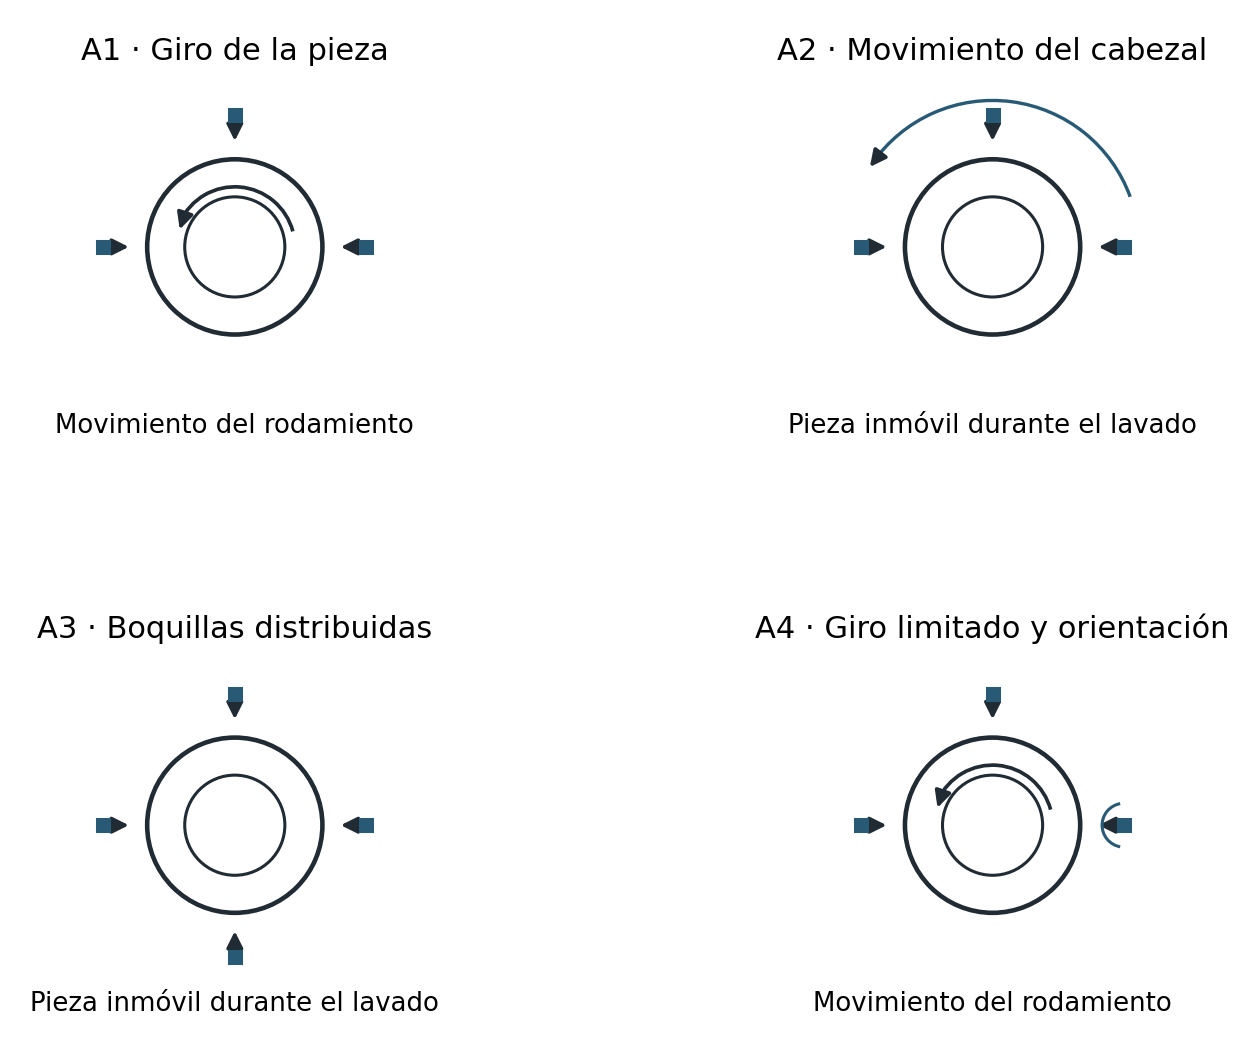
\includegraphics[width=0.94\textwidth]{images/alternativas_funcionales}
\caption{Principios de movimiento de las cuatro alternativas conceptuales. Elaboración propia.}
\label{fig:alternativas_revision}
\end{figure}

\subsection{Selección y trade-offs}

Las alternativas se compararon con una matriz de ocho criterios, pesos que suman uno y una escala de uno (condición desfavorable) a cuatro (muy favorable). Las notas expresan juicios de diseño basados en las funciones previstas; no equivalen a eficiencias medidas ni a probabilidades de falla. La seguridad recibió el mayor peso por la masa manipulada; la cobertura y la preservación, por su relación con la finalidad del lavado; energía y fluido, por las necesidades de accionamiento y aplicación; y fabricabilidad, mantenimiento y costo representaron la implementación. La Tabla~\ref{tab:matriz_revision} contiene las notas y el puntaje ponderado de cada alternativa.

\begin{table}[htbp]
\centering\small\singlespacing
\caption{Matriz ponderada de selección de la arquitectura}
\label{tab:matriz_revision}
\begin{tabular}{lccccc}
\toprule
\textbf{Criterio} & \textbf{Peso} & \textbf{A1} & \textbf{A2} & \textbf{A3} & \textbf{A4}\\
\midrule
Seguridad & 0,20 & 2 & 4 & 3 & 3\\
Cobertura & 0,17 & 3 & 4 & 3 & 4\\
Preservación & 0,15 & 2 & 4 & 4 & 3\\
Energía & 0,11 & 1 & 4 & 4 & 2\\
Fluido & 0,10 & 3 & 3 & 2 & 3\\
Fabricabilidad & 0,10 & 3 & 3 & 4 & 2\\
Mantenimiento & 0,09 & 3 & 3 & 4 & 2\\
Costo & 0,08 & 2 & 3 & 3 & 2\\
\midrule
\textbf{Resultado} & \textbf{1,00} & \textbf{2,35} & \textbf{3,63} & \textbf{3,35} & \textbf{2,79}\\
\bottomrule
\end{tabular}
\par\smallskip\footnotesize
Fuente: matriz de la etapa anterior del proyecto; se reproduce su cálculo. La nota de cobertura de A2 evalúa el alcance funcional del principio (superficies exteriores, caras y agujero con la pieza inmóvil), no una geometría concreta del aplicador.
\end{table}

El puntaje de cada alternativa se obtuvo multiplicando la nota de cada criterio por su peso y sumando los productos. Para A2, el cálculo fue
\[
\begin{aligned}
S_{A2}={}&0{,}20(4)+0{,}17(4)+0{,}15(4)+0{,}11(4)\\
&+0{,}10(3)+0{,}10(3)+0{,}09(3)+0{,}08(3)=3{,}63.
\end{aligned}
\]
Este resultado seleccionó A2 como arquitectura de desarrollo: el rodamiento permanece inmovilizado durante la aplicación del fluido y el aplicador realiza el movimiento de limpieza.

La comparación más cercana fue con A3. A2 obtuvo una ventaja de 0,28 puntos: sus mayores notas de seguridad, cobertura y uso de fluido aportaron 0,47 puntos, mientras que sus menores notas de fabricabilidad y mantenimiento descontaron 0,19. El compromiso consistió en aceptar un mecanismo de accionamiento del aplicador a cambio de no mover una masa de tres toneladas y de variar la trayectoria de las boquillas alrededor de la pieza. Como A2 y A3 recibieron la misma nota de costo, aumentar únicamente ese peso no invierte su orden, aunque reduce la distancia entre sus puntajes.

La materialización del principio A2 evolucionó durante el desarrollo: de un aplicador anular con lanza axial a un cabezal sobre monorriel y, finalmente, a una U superior giratoria con una lanza interior y un par de boquillas inferiores en cada brazo (Anexo~\ref{anx:iteraciones}). La misma lógica de decisión se aplicó en un segundo nivel al número de apoyos del bastidor (Anexo~\ref{anx:iteraciones}), al mecanismo de centrado (Sección~\ref{sec:seleccion-componentes}), al sistema de traslado y a la rueda (Sección~\ref{sec:seleccion-traslado-rueda}).

\subsection{Selección del sistema de traslado y de la rueda}
\label{sec:seleccion-traslado-rueda}

El traslado de la mesa cargada se planteó primero como empuje manual. Con la masa de diseño de 3500~kg, el empuje calculado fue de 325~N para arrancar en el escenario de diseño y de 837~N en el adverso, y la parada en 0,10~m exigía 565~N (Sección~\ref{sec:dimensionamiento-traslado}). Esas fuerzas superan la cifra guía de la HSE británica para iniciar o detener a mano una carga empujada, 200~N para hombres y 150~N para mujeres, que es un filtro de riesgo y no un límite \cite{hsepushpull}. Por eso el empuje directo, incluso con un freno, no pasó el filtro de ergonomía. Las demás opciones se compararon en una matriz ponderada que incluyó la disponibilidad de componentes en el mercado local (Tabla~\ref{tab:traslado-alternativas}).

\begin{table}[htbp]
\centering\small\singlespacing
\caption{Selección del sistema de traslado de la mesa}
\label{tab:traslado-alternativas}
\begin{tabularx}{\textwidth}{@{}Ycccccc>{\bfseries}c@{}}
\toprule
\textbf{Alternativa} & \textbf{Seg.} & \textbf{Conf.} & \textbf{Costo} & \textbf{Integr.} & \textbf{Oper.} & \textbf{Disp.} & \textbf{Total}\\
 & 0,25 & 0,20 & 0,20 & 0,15 & 0,10 & 0,10 & \\
\midrule
Empuje manual con freno & \multicolumn{7}{c}{No pasa el filtro: 325--837~N frente a 200~N} \\
Manivela en la mesa, rueda motriz & 4 & 3 & 4 & 2 & 3 & 4 & 3,40\\
Motorreductor en la mesa, rueda motriz & 4 & 2 & 2 & 1 & 5 & 3 & 2,75\\
Cable sin fin con motor fijo & 4 & 3 & 2 & 3 & 5 & 3 & 3,25\\
Cable sin fin con torno manual & 4 & 3 & 4 & 3 & 2 & 4 & 3,45\\
Doble cadena bajo la mesa, motorizada & 4 & 4 & 2 & 4 & 5 & 4 & 3,70\\
Doble cadena bajo la mesa, con volante & 5 & 4 & 4 & 4 & 3 & 5 & 4,25\\
\bottomrule
\end{tabularx}
\par\smallskip\footnotesize
Seg.: seguridad y ergonomía; Conf.: confiabilidad en ambiente húmedo; Integr.: integración sin modificar la mesa, las ruedas ni la puerta; Oper.: rapidez y repetibilidad; Disp.: disponibilidad local de componentes y mantenimiento. Puntajes de 1 a 5 asignados por los autores.
\end{table}

Se seleccionó la doble cadena bajo la mesa accionada con un volante fuera de la cabina, con 4,25 puntos. La segunda opción fue la misma cadena con motor, con 3,70. La diferencia está en el costo y la disponibilidad, a cambio de una operación más lenta: si el peso de la operación sube a 0,30, las dos cadenas empatan (3,99 y 3,97). Por ese resultado, la motorización se mantiene como mejora sobre la misma transmisión y se trata en las recomendaciones.

La rueda se revisó porque la versión anterior comparó la carga del estado límite último, de 26,62~kN, con la capacidad de rodadura a 4~km/h, de 24,52~kN, y obtuvo un exceso de 8,5\,\%. Esa capacidad corresponde al desgaste en servicio. Se separaron las dos comprobaciones y se compararon las ruedas de 200 y 250~mm del mismo fabricante (Tabla~\ref{tab:rueda-200-250}).

\begin{table}[htbp]
\centering\small\singlespacing
\caption{Comparación de las ruedas de 200 y 250 mm para la mesa de traslado}
\label{tab:rueda-200-250}
\begin{tabularx}{\textwidth}{@{}Yrr@{}}
\toprule
\textbf{Criterio} & \textbf{Rueda de 200 mm} & \textbf{Rueda de 250 mm}\\
\midrule
Capacidad de rodadura a 4~km/h \cite{blickle2026} & 24,52 kN & 39,23 kN\\
Capacidad estática \cite{blickle2026} & 61,29 kN & 98,07 kN\\
Servicio: 21,87 kN frente a la capacidad de rodadura & 0,89 & 0,56\\
Estado límite último: 26,62 kN frente a la capacidad estática & 0,43 & 0,27\\
Riel asignado y masa de los dos rieles \cite{arcelor2023} & A45; 289 kg & A55; 416 kg\\
Costo adicional respecto de la rueda de 200 mm & -- & S/~4230 (14\,\%)\\
Masa móvil adicional & -- & 56 kg\\
\bottomrule
\end{tabularx}
\par\smallskip\footnotesize
Rueda más cargada con la mesa en tres ruedas, masa de 3500~kg, excentricidad de 100~mm en ambas direcciones y factor de impacto de 1,15; la carga última aplica 1,40. El precio de la rueda de 250~mm se estimó por su masa.
\end{table}

Se mantuvo la rueda de 200~mm sobre riel A45. Cumple las dos comprobaciones con supuestos envolventes, mientras que la de 250~mm costaría unos S/~4230 más y obligaría a cambiar el riel, el eje y la horquilla. Falta que el fabricante confirme la capacidad a la velocidad de traslado de la mesa, muy inferior a los 4~km/h del catálogo.

\subsection{Criterios ambiental y social}
\label{sec:matriz-ambiental-social}

La matriz no separó criterios ambiental y social: sus efectos están en los criterios de fluido y energía, que miden el consumo y el efluente, y en el de seguridad, que mide la exposición del personal. El Capítulo~\ref{cap:seguridad-ambiente} los evalúa de forma cualitativa para la arquitectura seleccionada, de modo que el puntaje de A2 sustenta la arquitectura de desarrollo y no una comparación ambiental entre alternativas.

\section{Descripción general de los componentes o partes de la solución seleccionada}

La solución seleccionada realiza un lavado exterior del rodamiento completo, para su inspección visual, retirado del HPGR y apoyado horizontalmente con su eje vertical e inmóvil durante la aplicación del fluido, antes de desmontarlo por componentes. En esta primera etapa se tratan las superficies exteriores, las dos caras y la superficie accesible del agujero; no se busca limpiar los espacios internos entre rodillos y aros. La segunda etapa, conceptual y fuera del alcance de esta máquina, comprende la limpieza de los elementos desmontados (aros, rodillos y jaula) y de las zonas que el lavado no alcanza, como la franja que ocultan los topes de retención. Sus útiles y criterios de limpieza no se dimensionan ni evalúan en este proyecto.

El soporte es una mesa móvil con bastidor de perfiles W6$\times$9 que se extrae de la cabina para cargar el rodamiento con grúa. En la estación de carga se inserta el pasador de bloqueo y los centradores posicionan la pieza; luego una doble cadena accionada con un volante traslada la mesa sobre rieles hasta la estación de lavado, donde se bloquea de nuevo. Los tres apoyos sectoriales, a 0$^\circ$, 120$^\circ$ y 240$^\circ$ bajo la cara inferior del aro exterior, reciben la carga vertical; los centradores solo fijan la posición lateral y los topes retienen la pieza.

La aplicación se realiza con un distribuidor en U que gira a 1,7~rpm, alimentado por una unión rotativa y sostenido por un soporte superior, y con una lanza interior que entra por el agujero. En total hay 24 boquillas fijas: cada brazo de la U lleva dos superiores, cinco laterales y un par inferior de abanico estrecho, y la lanza lleva seis. La cabina contiene las salpicaduras y el líquido vuelve al tanque de lavado; el drenaje se representa en el esquema hidráulico, sin dimensionarse. La Tabla~\ref{tab:componentes_revision} relaciona cada conjunto con su función, el objetivo específico al que responde y la forma en que se dimensiona o verifica.

\begingroup
\small\singlespacing
\setlength{\parskip}{0pt}
\setlength{\tabcolsep}{4pt}
\renewcommand{\arraystretch}{1.1}
\begin{longtable}{@{}>{\raggedright\arraybackslash}p{2.8cm}>{\raggedright\arraybackslash}p{\dimexpr(\textwidth-2.8cm-6\tabcolsep)*38/100\relax}>{\raggedright\arraybackslash}p{\dimexpr(\textwidth-2.8cm-6\tabcolsep)*12/100\relax}>{\raggedright\arraybackslash}p{\dimexpr(\textwidth-2.8cm-6\tabcolsep)*50/100\relax}@{}}
\caption{Componentes de la solución seleccionada y su dimensionamiento}\label{tab:componentes_revision}\\
\toprule
\textbf{Conjunto} & \textbf{Función} & \textbf{OE} & \textbf{Dimensionamiento o verificación}\\
\midrule\endfirsthead
\caption[]{Componentes de la solución seleccionada y su dimensionamiento (continuación)}\\
\toprule
\textbf{Conjunto} & \textbf{Función} & \textbf{OE} & \textbf{Dimensionamiento o verificación}\\
\midrule\endhead
\midrule\multicolumn{4}{r}{\textit{Continúa en la página siguiente.}}\\\endfoot
\bottomrule\endlastfoot
Bastidor de perfiles & Recibir y transmitir las cargas. & OE4 & Modelo de barras, torsión no uniforme y uniones soldadas a momento.\\
Apoyos sectoriales y revestimiento & Apoyar el rodamiento y preservar la superficie de contacto. & OE4 & Reacciones por equilibrio y presión media.\\
Ruedas, rieles y pedestales & Rodar la mesa entre las estaciones de carga y lavado. & OE4 & Carga de rueda, fuerza lateral de guiado, viga del riel y anclajes.\\
Traslado por doble cadena & Mover y detener la mesa sin empuje directo. & OE3, OE4 & Matriz de selección, tiro de la cadena, eje y fuerza en el volante.\\
Centradores & Posicionar el rodamiento sin soportar su peso. & OE4, OE5 & Selección multicriterio, FEM local y error de colocación por nivel de fuerza.\\
Bloqueo y topes & Inmovilizar la mesa y retener la pieza. & OE4 & Pasador con ajuste H7/g6 y secuencia de operación.\\
Distribuidor en U, eje y cubo & Aplicar el fluido al exterior y a las dos caras. & OE4, OE5 & Huella, número de boquillas, CFD y verificación estructural.\\
Lanza interior & Aplicar el fluido al agujero y a la parte interior de la cara inferior. & OE4, OE5 & Visibilidad geométrica y CFD.\\
Soporte superior y accionamiento & Sostener el distribuidor y hacerlo girar con par limitado. & OE4 & Selección de catálogo y comprobaciones resumidas (Anexo~\ref{anx:calculos}).\\
Circuito hidráulico & Alimentar las 24 boquillas desde el tanque. & OE4 & Red iterativa, altura, potencia, NPSH y esquema hidráulico.\\
Cabina, tanques y drenaje & Contener, recoger y recircular el líquido. & OE4 & Representación en el CAD y en el esquema hidráulico, barridos y presupuesto; sin dimensionamiento.\\
\end{longtable}
\endgroup

El Capítulo~\ref{cap:diseno} desarrolla el dimensionamiento de cada conjunto con las ecuaciones del Capítulo~\ref{cap:marco-teorico}; el Capítulo~\ref{cap:resultados} somete el conjunto dimensionado a la verificación numérica frente a las especificaciones y las restricciones.
